\section*{Teoretická část}

Hlavním cílem této úlohy je změřit pohyblivost $\mu$ a koncentraci $n$ nositelů náboje ve vzorku polovodiče.
Měřený polovodič bude vzorek germania typu n, tedy majoritními nositeli náboje jsou elektrony.
Pohyblivost a koncentraci elektronů určíme ze změřené měrné vodivosti $\sigma$ a Hallovy konstanty $R_H$.

Použitý vzorek je tvaru hranolu s rozměry $t$, $d$ a $l$ a je opatřený šesti kontakty (viz obrázek \ref{obr:vzorek}).

\begin{figure}[htbp]
\centering
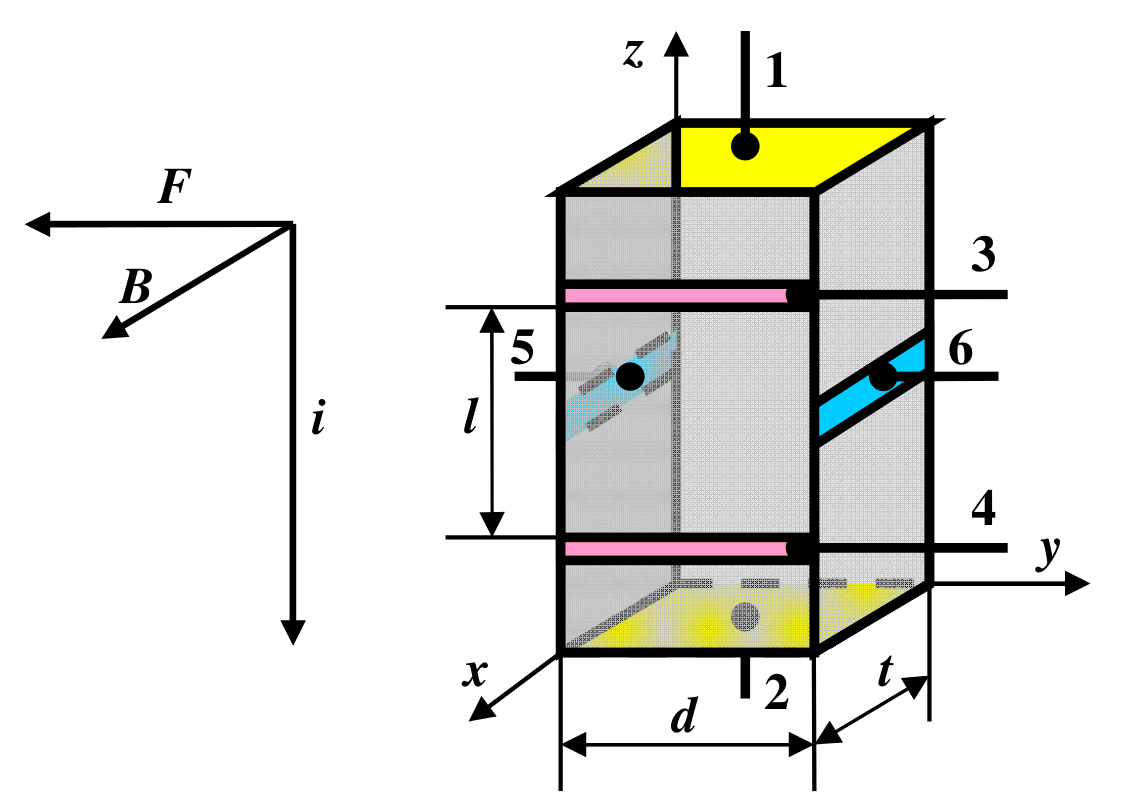
\includegraphics[width=100mm,scale=0.5]{graficos/vzorek}
\caption{Označení rozměrů a kontaktů na měřeném vzorku (převzato z \cite{skripta})}
\label{obr:vzorek}
\end{figure}

Měrnou vodivost vzorku určíme z naměřené voltampérové charakteristiky.
Vzorek zapojíme jako na obrázku \ref{obr:schemaodpor} a naměříme závislost $I_{12}$ na $U_{34}$.
Měrnou vodivost určíme z fitu
\begin{equation}
I_{12}=\sigma \frac{td}{l} U_{34} \,.
\end{equation}

\begin{figure}[htbp]
\centering
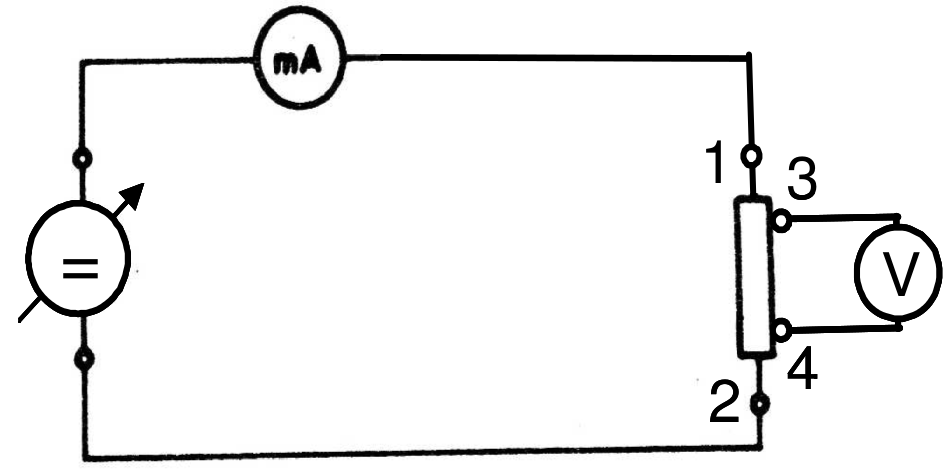
\includegraphics[width=100mm, scale=0.5]{graficos/schema}
\caption{Zapojení pro měření měrné vodivosti (převzato z \cite{skripta})}
\label{obr:schemaodpor}
\end{figure}

Pro měření Hallovy konstanty vložíme vzorek procházený proudem $I_{12}$ do pole o magnetické indukci $B$.
V důsledku působení magnetického pole na pohybující se elektrony ve vzorku se elektrony odchýlí a mezi kontakty 5 a 6 vznikne tzv. Hallovo napětí $U_H$.
Hallovo konstantu určíme z fitu \cite{skripta}
\begin{equation}
U_H=R_H\frac{I_{12} \cdot B}{t} \,.
\end{equation}

Vzhledem k tomu, že kontakty 5 a 6 nejsou s velkou pravděpodobností umístěny přesně symetricky, naměříme na nich při průchodu proudu vzorkem nenulové napětí i při nulové magnetické indukci.
Abychom tento jev eliminovali, změříme napětí při obou polaritách magnetického pole a správnou hodnotu $U_H$ určíme jako
\begin{equation}
| U_H |=|U_{56}^+ - U_{56}^-|/2 \,.
\end{equation}

Mezi $R_H$ a koncentrací $n$ platí vztah \cite{skripta}
\begin{equation} \label{eq:koncentrace}
R_H = \frac{r_H}{en} \,,
\end{equation}
kde $e$ je náboj elektronu a $r_H$ je tzv. rozptylový faktor.
V našem případě můžeme uvažovat $r_H = 3\pi/8$. \cite{skripta}

Ze známé $R_H$ a $\sigma$ můžeme vypočítat tzv. Hallovskou pohyblivost ze vztahu \cite{skripta}
\begin{equation} \label{eq:pohyblivost}
\mu = R_H \sigma \,.
\end{equation}

Magnetické pole budeme realizovat elektromagnetem.